\documentclass{beamer}
\usepackage[T1]{fontenc}
\usepackage[utf8]{inputenc}
\usepackage[cyr]{aeguill}
\usepackage[english]{babel}
\usepackage{amsmath,amssymb,amsthm}
\usepackage{bm}
\usepackage{graphicx}
\usepackage{geometry}
\usepackage{tikz}
\usepackage{diffcoeff}
\usepackage{tcolorbox}
\usepackage{color}

%\usepackage{natbib}

\graphicspath{{./Figures/}}

\mode<presentation> {
	%\usetheme{Singapore}
	\usetheme{Madrid}
}
\usefonttheme{serif}
\usecolortheme{beaver}

\DeclareMathOperator*{\argmax}{arg\,max}
\DeclareMathOperator*{\argmin}{arg\,min}

\newcommand{\matr}[1]{\bm{#1}} 

% make bibliography entries smaller
%\renewcommand\bibfont{\scriptsize}
% If you have more than one page of references, you want to tell beamer
% to put the continuation section label from the second slide onwards
%\setbeamertemplate{frametitle continuation}[from second]
% Now get rid of all the colours
%\setbeamercolor*{bibliography entry title}{fg=black}
%\setbeamercolor*{bibliography entry author}{fg=black}
%\setbeamercolor*{bibliography entry location}{fg=black}
%\setbeamercolor*{bibliography entry note}{fg=black}
% and kill the abominable icon
%\setbeamertemplate{bibliography item}{}


\expandafter\def\expandafter\insertshorttitle\expandafter{%
	\insertshorttitle\hfill%
	\insertframenumber\,/\,\inserttotalframenumber}

%
%\addtobeamertemplate{frametitle}{}{
%	\vskip-1em
%	\begin{tikzpicture}[remember picture,overlay]
%	\node[anchor=north east,yshift=-10pt] at (current page.north east) {
\includegraphics[height=0.8cm]{ISAE-SUPAERO.png}};
%	\end{tikzpicture}
%}

\title[INFIDHEM Workshop]{PH formulation for thin and thick plates}
\author[A. Brugnoli ISAE-SUPAERO]{\small Andrea Brugnoli}
%\date{23 janvier 2014}

% Clear the navigation bar
\setbeamertemplate{navigation symbols}{}
%\setbeamercolor{section in head/foot}{fg=black, bg=white} 

\AtBeginSection[]{
	\begin{frame}{Plan}
	\small \tableofcontents[currentsection, currentsubsection]
\end{frame} 
}


\begin{document}
	
\begin{frame}
	\titlepage
\begin{columns}
	\begin{column}{0.5\textwidth}
		\centering
		
\includegraphics[height=0.2\textheight]{ISAE-SUPAERO.PNG}
	\end{column}
	\begin{column}{0.5\textwidth}
		\centering
		
\includegraphics[scale=0.3]{infidhem.png}
	\end{column}
\end{columns}

\end{frame}

\begin{frame}
\frametitle{Plan}
\small
\tableofcontents
\normalsize
\end{frame}

\section{Me and my thesis}

\begin{frame}{}
\frametitle{Me}

\textbf{Formation:}
\begin{itemize}
	\item High school diploma in Humanities, \textbf{Vérone};
	\item Bachelor in Mechanical Engineering, Politecnico di Milano, \textbf{Milan};
	\item Master of science in Space Engineering, Politecnico di Milano, \textbf{Milan};
	\item Double Degree Politecnico/Isae-SUPAERO, \textbf{Toulouse};
	\item Research Master in Automatic Control, Université Paris Saclay/\,Supélec, \textbf{Paris/Toulouse};
\end{itemize}
\centering
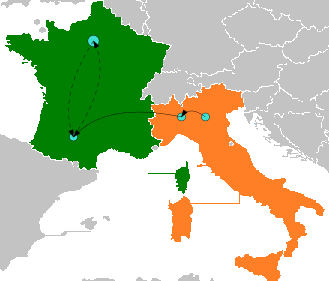
\includegraphics[height=0.4\textheight]{trip.png}

\end{frame}

\begin{frame}{PHD title and purposes}

\begin{block}{PHD title}
Modeling and control by the Port-Hamiltonian formalism of 2D flexible structures with varying boundary conditions.
\end{block}
\begin{block}{Supervisors}
Daniel Alazard \hspace{1.5cm} Valerie Budinger 
\hspace{1.5cm}
Denis Matignon
\end{block}
\begin{block}{Fundings}
This work is funded by ISAE-SUPAERO.
\end{block} 

\begin{block}{Objectives}
Patran/Nastran cannot model  flexible structures with a priori unknown boundary conditions. The PH framework can overcome this problem, making possible the analysis of system even when boundary conditions are unknown. Moreover, we aim to examine performance specifications in the PH formalism.
\end{block}

\end{frame}

\section{The 1D case: Euler-Bernoulli and Timoshenko beams}

\begin{frame}{The corresponding 1D models}
\begin{columns}
	\begin{column}[t]{0.45\textwidth}
		\begin{block}{Euler-Bernoulli beam}
			\begin{itemize}
				\item Valid for thin beams \\
				\item Dimension of the PH model: 2 \\
				\item Differential operator $J$ of order 2 \\
			\end{itemize}
		\end{block}
	\begin{equation*}
	\begin{aligned}
	\bm{\alpha} &= [\rho v, \ \diffp[2]{w}{x}]^T \\
	\bm{e} &= [v, \ M_{xx}]^T \\
	J &= 
	\begin{pmatrix}
	0 &  -\diffp[2]{}{x} \\
	\diffp[2]{}{x} & 0  \\
	\end{pmatrix}
	\end{aligned}
	\end{equation*}
	\end{column}
	\begin{column}[t]{0.5\textwidth}
		\begin{block}{Timoshenko beam}
			\begin{itemize}
				\item Valid for thick beams \\
				\item Dimension of the PH model: 4 \\
				\item Differential operator $J$ of order~1 \\
			\end{itemize}
		\end{block}
	\begin{equation*}
	\begin{aligned}
	\bm{\alpha} &= [\rho v, \ I_{\rho} \omega_x, \ \diffp{w}{x} - \phi_x, \ \diffp{\phi_x}{x}]^T \\
	\bm{e} &= [v, \ \omega_x, \ T_x, \ M_{xx} ]^T \\
	J &= 
	\begin{pmatrix}
	0 & 0 &  \diffp{}{x} & 0 \\
	0 & 0 &  1 & \diffp{}{x} \\
	\diffp{}{x} & -1 & 0 & 0  \\
	0 & \diffp{}{x} & 0 & 0 \\
	\end{pmatrix}	
	\end{aligned}
	\end{equation*}
	\end{column}
\end{columns}
\end{frame}

\section{Kirchhoff-Love theory}

\begin{frame}{Model Hypothesis}
\begin{tcolorbox}
	\textit{Plane cross sections remains plane and normal to the middle-plane during deformations.} 
	\begin{figure}
		\centering
		\includegraphics[height=0.4\textheight]{Kirchh_sketch.eps}
	\end{figure}	
\end{tcolorbox}

Consequently the displacement field assumes the following expression
\begin{equation*}
u(x,y,z) = -z \diffp{w}{x} \qquad v(x,y,z) = -z \diffp{w}{y} \qquad 
w(x,y,z) = w(x,y)
\end{equation*}
\end{frame}

\begin{frame}{Constitutive relations}

Plane strain condition
\begin{equation*}
\bm{\epsilon} =  
\begin{pmatrix}
\epsilon_{xx} \\
\epsilon_{yy} \\
\gamma_{xy} \\
\end{pmatrix}  = 
\begin{pmatrix}
\diffp{}{x} & 0 \\
0 & \diffp{}{y} \\
\diffp{}{y} & \diffp{}{x} \\
\end{pmatrix}
\begin{pmatrix}
-z \diffp{w}{x}\\
-z \diffp{w}{y}\\
\end{pmatrix} = 
-z
\begin{pmatrix}
\diffp[2]{w}{x} \\
\diffp[2]{w}{y} \\
2 \diffp{w}{x,y} \\
\end{pmatrix} = -z
\begin{pmatrix}
\kappa_{xx} \\
\kappa_{yy} \\
\kappa_{xy} \\
\end{pmatrix} = -z \bm{\kappa}
\end{equation*}

Generalized momenta
\begin{equation*}
\bm{M} =
\begin{pmatrix}
M_{xx} \\
M_{yy} \\
M_{xy} \\
\end{pmatrix} = \int_{-\frac{h}{2} }^{\frac{h}{2}}
-z \bm{\sigma} dz \bm{\kappa} =
\int_{-\frac{h}{2} }^{\frac{h}{2}}
E z^2 dz \bm{\kappa}= \bm{D} \bm{\kappa}
\end{equation*}
\begin{equation*}
	\matr{D} = 
	\int_{-\frac{h}{2} }^{\frac{h}{2}}
	E z^2 dz = D 
	\begin{bmatrix}
	1 & \nu & 0 \\ 
	\nu & 1 & 0 \\
	0    & 0 & \frac{1}{2} (1 - \nu)
	\end{bmatrix}
\end{equation*}
where $D = \frac{E h^3}{12 (1 - \nu)}$ is the flexural stiffness and $\nu$ is the Poisson ratio.
\end{frame}



\begin{frame}{Variational description}
Constitutive relations (physical parameters, namely $D, \nu$ do not depend on $z$ but may depend on $x, y$)
\begin{equation*}
\begin{aligned}
\kappa_{xx} & =\diffp[2]{w}{x} \\
\kappa_{yy} & =\diffp[2]{w}{y} \\
\kappa_{xy} & =2 \diffp{w}{x,y} \\
\end{aligned} \qquad
\begin{aligned}
M_{xx} & =D\left(\diffp[2]{w}{x} + \nu \diffp[2]{w}{y}\right)\\
M_{yy} & =D\left(\diffp[2]{w}{y} + \nu \diffp[2]{w}{x}\right)\\
M_{xy} & =D (1 - \nu) \diffp{w}{x,y} \\
\end{aligned}
\end{equation*}


The Euler-Lagrange equations arise form the following extrema problem (where $\mathcal{V}$ is a suitable functional space):
\begin{align*} 
w_0 &= \{w \in \mathcal V; \; \left.\delta F(w) \right|_{w_0} = 0\}  \\
F(w) &= \int_0^T \int_\Omega \left\{\mathcal{K} - \mathcal{U} + \mathcal{W} \right\} d\Omega \, dt
\end{align*}


\end{frame}

\begin{frame}{Euler Lagrange equations}

Work and energy densities defined by:
\begin{align*}
\mathcal{W} &= pw \qquad &\text{Work of external forces}  \\
\mathcal{K} &= \frac{1}{2} \mu \left(\diffp{w}{t}\right)^2  \qquad &\text{Kinetic energy}\\
\mathcal{U} &=  \frac{1}{2} \bm{\kappa}^T \matr{D} \bm{\kappa}  \qquad &\text{Deformation energy}	
\end{align*} 


\begin{block}{Euler-Lagrange equation for the Kirchhoff plate}
	\begin{equation*}
	\mu \diffp[2]{w}{t}  + \diffp[2]{M_{xx}}{x} + 2 \diffp{M_{xy}}{x,y} + \diffp[2]{M_{yy}}{y}= p
	\end{equation*}
\end{block}
In the homogeneous case ($D, \nu$ constant) the ruling equation is
\begin{equation*}
\mu \diffp[2]{w}{t}  + D \Delta^2 w= p
\end{equation*}
In the sequel it is assumed $p=0$.
\end{frame}

\section{PH formulation of the Kirchhoff plate} 

\begin{frame}{Energy and co-energy variables}
This model is the 2D extension of the Bernoulli beam. It is logical to select as energy variable the linear momentum, together with the curvatures

\begin{equation*}
\bm{\alpha} = (\mu v,\ \kappa_{xx},\ \kappa_{yy},\ \kappa_{xy})^T
\end{equation*}

where $v = \diffp{w}{t}$. The Hamiltonian density is given by 
\begin{equation*}
\mathcal{H} = \mathcal{K} + \mathcal{U} = \frac{1}{2} \bm{\alpha}^T \begin{bmatrix}
\frac{1}{\mu} & 0 \\
0 & \bm{D} \\
\end{bmatrix} \bm{\alpha}
\end{equation*}

So the variational derivative of the total Hamiltonian $H = \int_{\Omega} \mathcal{H} \ d\Omega$ provides as co-energy variables
\begin{equation*}
\mathbf{e} := \diffd{H}{\bm{\alpha}} = (v,\ M_{xx},\ M_{yy},\ M_{xy})^T
\end{equation*}
 
\end{frame}



\begin{frame}{Definition of J and boundary variables}
The skew-adjoint operator relating energies and co-energies is found to be 
\begin{equation*}
J = 
\begin{bmatrix}
0 & -\diffp[2]{}{x} & -\diffp[2]{}{y} & - 2 \diffp{}{x,y}\\
\diffp[2]{}{x} & 0 & 0 & 0 \\
\diffp[2]{}{y} & 0 & 0 & 0 \\
2 \diffp{}{x,y} & 0 & 0 & 0 \\
\end{bmatrix} 	\qquad
\diffp{\bm{\alpha}}{t} = J \mathbf{e} 
\end{equation*}
\begin{tcolorbox}
	The boundary variables are obtained by evaluating the time derivative of the Hamiltonian
	\begin{multline*}
	\dot{H} = \int_\Omega \diffd{H}{\bm{\alpha}}   \cdot \diffp{\bm{\alpha}}{t} \; d\Omega = \int_\Omega \left\{ e_1 \left(-\diffp[2]{e_2}{x} -\diffp[2]{e_3}{y} - 2 \diffp{e_4}{x,y} \right) \right. \\ \left. + e_2 \diffp[2]{e_1}{x} + e_3 \diffp[2]{e_1}{y} + 2 e_4 \diffp{e_1}{x,y}  \right\} d\Omega
	\end{multline*}
\end{tcolorbox}



\end{frame}

\begin{frame}
By Green thm, equivalent results are found due to the \textcolor{red}{mixed derivative}:
\begin{multline*}
\dot{H} = \int_{\partial \Omega} \left\{ n_x \left(\textcolor{blue}{ e_2 \diffp{e_1}{x} - e_1 \diffp{e_2}{x} }  \textcolor{red}{+ 2 e_4 \diffp{e_1}{y}} \right) \right.\\ \left. + n_y \left(\textcolor{blue}{e_3 \diffp{e_1}{y} - e_1 \diffp{e_3}{y}} \textcolor{red}{-2 e_1 \diffp{e_4}{x} } \right) \right\} ds
\end{multline*}	
\begin{multline*}
\dot{H} = \int_{\partial \Omega} \left\{ n_x \left(\textcolor{blue}{ e_2 \diffp{e_1}{x} - e_1 \diffp{e_2}{x} } \textcolor{red}{ - 2 e_1 \diffp{e_4}{y} }\right) \right.\\ \left. + n_y \left( \textcolor{blue}{ e_3 \diffp{e_1}{y} - e_1 \diffp{e_3}{y} } \textcolor{red}{ + 2 e_4 \diffp{e_1}{x}}\right) \right\} ds
\end{multline*}
\begin{tcolorbox}
	\centering
	\includegraphics[width=0.75\textwidth]{Plate_ref.eps}
\end{tcolorbox}
\end{frame}

\begin{frame}{}
The half-sum of both terms does restore symmetry 
\begin{align*}
\dot{H} = \int_{\partial \Omega}  & \left\{  n_x \left(e_2 \diffp{e_1}{x}  + e_4 \diffp{e_1}{y}  - e_1 \diffp{e_2}{x} - e_1 \diffp{e_4}{y}\right)
\right. \nonumber \\
&   \left. +n_y \left(e_3 \diffp{e_1}{y} + e_4 \diffp{e_1}{x} - e_1 \diffp{e_3}{y} - e_1 \diffp{e_4}{x} \right) \right\} ds
\end{align*}
If the physical variables are introduced 
\begin{align*}
\dot{H} = \int_{\partial \Omega}  & \left\{  n_x \left(M_{xx} \diffp{v}{x} + M_{xy} \diffp{v}{y} - v \, \diffp{M_{xx} }{x}   - v \, \diffp{M_{xy}}{y}\right)
\right.  \nonumber\\
&  \left. +n_y \left(M_{yy} \diffp{v}{y} + M_{xy} \diffp{v}{x} - v \, \diffp{M_{yy}}{y} - v\, \diffp{M_{xy}}{x} \right) \right\} ds
\end{align*}

\end{frame}

\begin{frame}
The boundary forces and momenta need to be defined:
\begin{equation*}
\label{eq:QnMnnMns}
\begin{aligned}
\text{Shear Force} \; \; \quad \textcolor{blue}{Q_{n}} &:= n_x Q_x + n_y Q_y   \\
\text{Flexural momentum} \quad 
\textcolor{blue}{M_{nn}} &:= \bm{n}^T	
\begin{pmatrix}
M_{xx} n_x + M_{xy} n_y \\
M_{xy} n_x + M_{yy} n_y \\
\end{pmatrix} \qquad 
\bm{n} = 
\begin{pmatrix}
n_x \\
n_y \\
\end{pmatrix}
\\
\text{Torsional momentum} \quad \textcolor{blue}{M_{ns}} &:= \bm{s}^T	
\begin{pmatrix}
M_{xx} n_x + M_{xy} n_y \\
M_{xy} n_x + M_{yy} n_y \\
\end{pmatrix} \qquad 
\bm{s} = 
\begin{pmatrix}
-n_y \\
n_x \\
\end{pmatrix}
\end{aligned}
\end{equation*}
where $Q_x = - \diffp{M_{xx}}{x} -\diffp{M_{xy}}{y}$ and $\; Q_y = - \diffp{M_{yy}}{y} -\diffp{M_{xy}}{x}$.

\begin{tcolorbox}
\centering
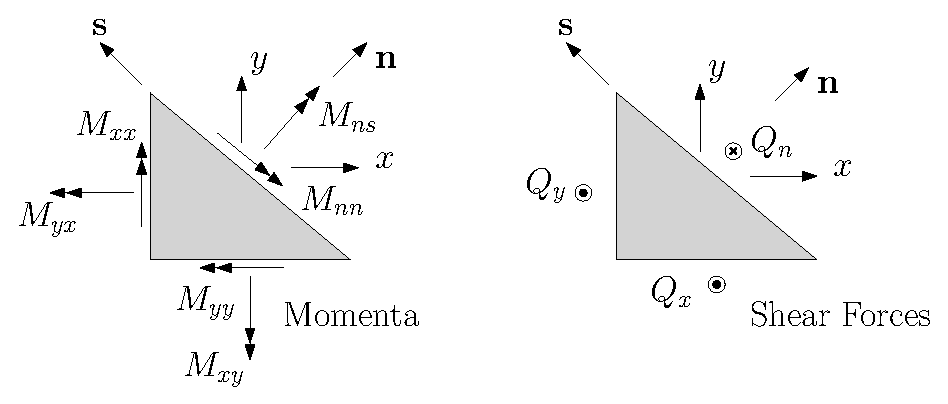
\includegraphics[width=0.7\textwidth]{Cauchy_law.eps}
\end{tcolorbox}
\end{frame}

\begin{frame}
Using the previous definition of $Q_n$ into the energy balance
\begin{align*}
\dot{H} = \int_{\partial \Omega}  & \left\{ 
\begin{pmatrix}
\diffp{v}{x} & \diffp{v}{y} \\
\end{pmatrix}
\begin{pmatrix}
M_{xx} n_x + M_{xy} n_y \\
M_{xy} n_x + M_{yy} n_y \\
\end{pmatrix} 
+ v Q_n
\right\} ds
\end{align*}
To get the proper boundary conditions the gradient of the vertical velocity has to be projected along the normal and tangential direction
\begin{equation*}
\nabla v = \left(\nabla v^T \bm{n} \right) \,\bm{n} + \left(\nabla v^T \bm{s} \right) \, \bm{s} = \diffp{v}{n} \; \bm{n} +   \diffp{v}{s} \; \bm{s}
\end{equation*}
So the time derivative of the Hamiltonian can be finally written as
\begin{equation*}
\dot{H} = \int_{\partial \Omega} \left\{ v \, Q_n + \diffp{v}{s} \, M_{ns} + \diffp{v}{n} \, M_{nn}\right\} ds
\end{equation*}

\textcolor{red}{Variables $v, \diffp{v}{\bm{s}}$ are kinematically related}. Another integration by part is needed to highlight the power conjugated variables. Given a closed and regular boundary the integration by parts leads to
\begin{equation*}
\int_{\partial \Omega} \diffp{v}{s} \, M_{ns} = - \int_{\partial \Omega} \diffp{M_{ns}}{s} \, v
\end{equation*}
\end{frame}

\begin{frame}{Final energy balance and boundary variables}
\begin{tcolorbox}
 The energy balance can be finally written as
\begin{equation*}
\label{eq:energyBal_Kir}
\dot{H} = \int_{\partial \Omega} \left\{ \textcolor{red}{v} \, \textcolor{blue}{\tilde{Q}_n} + \textcolor{red}{\diffp{v}{n}} \, \textcolor{blue}{M_{nn}} \right\} ds
\end{equation*} 
where $\textcolor{blue}{\tilde{Q}_n} = Q_n - \diffp{M_{ns}}{s}$ is the effective shear force.
\end{tcolorbox}

This energy balance highlights the power conjugated variables between input and output ports. No a priori causality is imposed. \\
\vspace{5mm}
Indeed this formulation enables us to consider different boundary conditions
\end{frame}

\subsection{Underlying Stokes-Dirac structure}
\begin{frame}{Functional spaces}
A possible choice for the flow space $\mathcal{F}$ is the space of the squared integrable function on the open bounded set $\Omega$, i.e $L^2(\Omega, \mathbb{R}^4)$. \\
\vspace{5mm}
For the effort space $\mathcal{E}$ a subset of the Sobolev space $H^2(\Omega, \mathbb{R}^4) \,$ is a possible choice. \\
\vspace{5mm}
The space of boundary conditions is found by considering the previous energy balance 

\begin{equation*}
\mathcal{Z} = \{z | \, z = B_{\partial}(e), \forall \, e \in \mathcal{E} \}  \qquad z = \left( \textcolor{blue}{V_n}, \textcolor{red}{v}, \textcolor{blue}{M_{nn}}, \textcolor{red}{\diffp{v}{n}} \right)^T 
\end{equation*}

The operator $B_{\partial}$ is a differential operator which contains derivatives and normal to retrieve the conjugated variable at the boundary. It is not simply a trace operator of the effort variables. It also involves the derivatives, both normal and tangential. 

\end{frame}
 
\begin{frame}{Stokes-Dirac structure}
 \begin{theorem}
	The set
	\begin{equation*}
	\mathbb{D} := \left\{ (f,e,z) \in \mathcal{F}\times\mathcal{E}\times\mathcal{Z} \; | \; f= - \diffp{\bm{\alpha}}{t} = -Je, z= B_{\partial}(e) \right\}
	\end{equation*} 
	is a Stokes-Dirac structure with respect to the pairing
	\begin{equation*}
	\ll (f_1, e_1, z_1), (f_2, e_2, z_2) \gg  \,= \int_{\Omega} \left[ e_1^T f_2 + e_2^T f_1 \right] d\Omega  + \int_{\partial \Omega} B_J(z_1, z_2) ds
	\end{equation*}
	where $B_J$ is a symmetric operator, arising from the application of the Green theorem. It reads
	\begin{equation*}
	B_J = 
	\begin{bmatrix}
	0 & 1 & 0 & 0 \\
	1 & 0 & 0 & 0 \\
	0 & 0 & 0 & 1 \\
	0 & 0 & 1 & 0 \\ 
	\end{bmatrix} \qquad
	\begin{aligned}
	B_J(z_1,z_2)= \tilde{Q}_{n,2} v_1 + M_{nn, 2} \diffp{v_1}{n} \\
	+ \tilde{Q}_{n,1} v_2 + M_{nn, 1} \diffp{v_2}{n}
	\end{aligned}
	\end{equation*}
\end{theorem}

\end{frame}

\section{Mindlin theory for thick plates}

\begin{frame}{Constitutive Relations}
Deflection of the cross section about $x$ : $\psi_y$  \\
Deflection of the cross section about $y$ : $-\psi_x$  
\begin{equation*}
u(x,y,z) = -z \psi_x \qquad v(x,y,z) = -z \psi_y \qquad 
w(x,y,z) = w(x,y)
\end{equation*}
The strain field can be separated into the bending and a shear part $\bm{\epsilon} = \left(\bm{\epsilon}_b, \; \bm{\epsilon}_s \right)^T$
\begin{equation*}
\bm{\epsilon}_b = 
\begin{pmatrix}
\epsilon_{xx} \\
\epsilon_{yy} \\
\gamma_{xy} \\
\end{pmatrix} = -z
\begin{pmatrix}
\diffp{\psi_x}{x} \\
\diffp{\psi_y}{y} \\
\diffp{\psi_y}{x} + \diffp{\psi_x}{y} \\
\end{pmatrix} = -z
\begin{pmatrix}
\kappa_{xx} \\
\kappa_{yy} \\
\kappa_{xy} \\
\end{pmatrix} = -z \bm{\kappa}
\end{equation*}

\begin{equation*}	
\bm{\epsilon}_s = 
\begin{pmatrix}
\gamma_{xz} \\
\gamma_{yz} \\
\end{pmatrix} = 
\begin{pmatrix}
\diffp{w}{x} - \psi_x \\
\diffp{w}{y} - \psi_y \\
\end{pmatrix}
\end{equation*}

\end{frame}

\begin{frame}{}
The stresses are split in the same manner
\begin{equation*}
\bm{\sigma} = 
\begin{pmatrix}
\bm{\sigma}_b \\
\bm{\sigma}_s \\
\end{pmatrix} = 
\begin{bmatrix}
E_b & 0 \\
0 & E_s \\
\end{bmatrix}
\begin{pmatrix}
\bm{\epsilon}_b \\
\bm{\epsilon}_s \\
\end{pmatrix}
\qquad
\bm{\sigma}_b = 
\begin{pmatrix}
\sigma_{xx} \\
\sigma_{yy} \\
\sigma_{xy} \\
\end{pmatrix}
\qquad
\bm{\sigma}_s = 
\begin{pmatrix}
\sigma_{xz} \\
\sigma_{yz} \\
\end{pmatrix}
\end{equation*}
The stresses integrated along the thickness generate momenta and forces
\begin{equation*}
\begin{pmatrix}
\bm{M} \\
\bm{Q} \\
\end{pmatrix} = \int_{-\frac{h}{2} }^{\frac{h}{2}}
\begin{pmatrix}
-z \bm{\sigma}_b \\
\bm{\sigma}_s \\
\end{pmatrix} dz=
\begin{bmatrix}
\bm{D}_b & 0 \\
0 & \bm{D}_s \\
\end{bmatrix}
\begin{pmatrix}
\bm{\kappa} \\
\bm{\epsilon}_s \\
\end{pmatrix}
\end{equation*}
Matrices $\bm{D}_b, \bm{D}_s$ come from the integration along the fiber of the constitutive relation
\begin{equation*}
\bm{D}_b = \int_{-\frac{h}{2} }^{\frac{h}{2}} z^2 E_b \; dz \qquad
\bm{D}_s = \int_{-\frac{h}{2} }^{\frac{h}{2}} z^2 E_s \; dz
\end{equation*}

\end{frame}

\begin{frame}
Since the kinematic model of the plate is too stiff, a correction factor is introduced inside matrix $\overline{\bm{D}}_s = k \bm{D}_s$. \\
\vspace{5mm}
If the mechanical properties are constant along the $z$ axis (but not necessarily in the $x, y$ plane), momenta and shear forces are given by
\begin{equation*}
\begin{aligned}
M_{xx} & =D\left(\diffp{\psi_x}{x} + \nu \diffp{\psi_y}{y}\right)\\
M_{yy} & =D\left(\diffp{\psi_y}{y} + \nu \diffp{\psi_x}{x}\right)\\
M_{xy} & =D \frac{(1 - \nu)}{2} \left(\diffp{\psi_x}{x} + \diffp{\psi_y}{y}\right) \\
\end{aligned} \qquad
\begin{aligned}
Q_{x} & =k G h \left(\diffp{w}{x} - \psi_x \right) \\
Q_{y} & =k G h \left(\diffp{w}{y} - \psi_y \right) \\
\end{aligned}
\end{equation*}

\end{frame}


\begin{frame}{Variational formulation}

These preliminary definitions allow defining the following extrema problem
\begin{equation*} 
\{w_0, \psi_{x, 0}, \psi_{y, 0}\} = \{w, \psi_x, \psi_y \in \mathcal V; \; \left.\delta F(w,\psi_x, \psi_y) \right|_{w_0, \psi_{x, 0}, \psi_{y, 0}} = 0\} 
\end{equation*}
\begin{multline*}
F(w, \psi_x, \psi_y) = \int_0^T \int_\Omega \left\{\mathcal{K} - \mathcal{U} + \mathcal{W} \right\} d\Omega \, dt =  \int_0^T  \int_\Omega \left\{ \frac{1}{2} \rho \left[ h \left(\diffp{w}{t}\right)^2 + \right.  \right. \\
\left. \left. \frac{h^3}{12}\left(\diffp{\psi_x}{t}\right)^2 + \frac{h^3}{12}\left(\diffp{\psi_y}{t}\right)^2 \right]  - \frac{1}{2}\bm{\kappa}^T \bm{D}_b \bm{\kappa} - \frac{1}{2}\bm{\epsilon}_s^T \bm{D}_s \bm{\epsilon}_s + pw \right\}  d\Omega \, dt
\end{multline*}


\end{frame}


\begin{frame}{Euler Lagrange Equations}
Work and energy densities defined by
\begin{align*}
\mathcal{W} =& pw &\text{Work}\\
\mathcal{K} =& \frac{1}{2} \rho \left[ h \left(\diffp{w}{t}\right)^2 +  \frac{h^3}{12}\left(\diffp{\psi_x}{t}\right)^2 + \frac{h^3}{12}\left(\diffp{\psi_y}{t}\right)^2 \right] &\text{Kinetic energy}\\
\mathcal{U} =& \frac{1}{2}\bm{\kappa}^T \bm{D}_b \bm{\kappa} + \frac{1}{2}\bm{\epsilon}_s^T \bm{D}_s \bm{\epsilon}_s  &\text{Deformation energy}	
\end{align*} 

\begin{block}{Euler Lagrange equations for the Mindlin plate}
	\begin{equation*}
	\begin{aligned}
	\rho h \diffp[2]{w}{t} &= p + \diffp{Q_x}{x} + \diffp{Q_y}{y} \\
	\rho\frac{h^3}{12} \diffp[2]{\psi_x}{t} &= Q_x + \diffp{M_{xx}}{x} + \diffp{M_{xy}}{y} \\
	\rho\frac{h^3}{12} \diffp[2]{\psi_y}{t} &= Q_y + \diffp{M_{xy}}{x} + \diffp{M_{y}}{y} \\
	\end{aligned}
	\end{equation*}
\end{block}

\end{frame}

\section{PH formulation of the Mindlin plate (Macchelli et al. 2005)}

\begin{frame}{Energies and co-energies variables}
Linear momenta and curvature are taken as energy variables. Additional the shear strain are considered, leading to 
\begin{equation*}
\bm{\alpha} = \left(\rho h v,\ \rho \frac{h^3}{12} \omega_x,\ \rho \frac{h^3}{12} \omega_y,\ \kappa_{xx},\ \kappa_{yy},\ \kappa_{xy},\ \gamma_{xz},\ \gamma_{yz} \right)^T
\end{equation*}
where $v = \diffp{w}{t},\ \omega_x = \diffp{\psi_x}{t},\ \omega_y = \diffp{\psi_y}{t}$. The Hamiltonian density is quadratic in the energy variables

\begin{equation*}
\mathcal{H} = \frac{1}{2} \bm{\alpha}^T \begin{bmatrix}
\frac{1}{\rho h} & 0 & 0 & 0 & 0 \\
0 & \frac{12}{\rho h^3} & 0 & 0 & 0 \\
0 & 0 & \frac{12}{\rho h^3} & 0 & 0 \\
0 & 0 & 0 & \bm{D}_b & 0 \\
0 & 0 & 0 &  0 & \bm{D}_s \\
\end{bmatrix} \bm{\alpha} 
\end{equation*}

The variational derivative provides as co-energy variables
\begin{equation*}
\mathbf{e} := \diffd{H}{\bm{\alpha}} = (v,\ \omega_x, \ \omega_y,\ M_{xx},\ M_{yy},\ M_{xy},\ Q_x, \ Q_y)^T
\end{equation*}
\end{frame}

\begin{frame}{Definition of J and boundary variables}
The skew-adjoint operator relating energies and co-energies is found to be
\begin{equation*}
J = 
\begin{bmatrix}
0 & 0 & 0 & 0 & 0 & 0 & \diffp{}{x} & \diffp{}{y} \\
0 & 0 & 0 & \diffp{}{x} & 0 & \diffp{}{y} & 1 & 0 \\
0 & 0 & 0 & 0 & \diffp{}{y} & \diffp{}{x} & 0 & 1 \\
0 & \diffp{}{x} & 0 & 0 & 0 & 0 & 0 & 0\\
0 & 0 & \diffp{}{y} & 0 & 0 & 0 & 0 & 0\\
0 & \diffp{}{y} & \diffp{}{x} & 0 & 0 & 0 & 0 & 0\\
\diffp{}{x} & -1 & 0 & 0 & 0 & 0 & 0\\
\diffp{}{y} & 0 & -1 & 0 & 0 & 0 & 0 & 0\\
\end{bmatrix} 	\qquad
\diffp{\bm{\alpha}}{t} = J \mathbf{e}
\end{equation*}
\end{frame}

\begin{frame}{Energy Balance}
The boundary variables are found by evaluating the time derivative of the Hamiltonian
\begin{multline*}
\dot{H} = \int_\Omega\left\{v \left(\diffp{Q_x}{x} + \diffp{Q_y}{y}\right) + \omega_x \left(Q_x + \diffp{M_{xx}}{x} + \diffp{M_{yy}}{y} \right) \right. \\
\left.  + \omega_y \left(Q_y + \diffp{M_{xy}}{x} + \diffp{M_{yy}}{y} \right)  + M_{xx} \diffp{\omega_x}{x} + M_{yy} \diffp{\omega_y}{y} \right. \\
\left. + M_{xy} \left(\diffp{\omega_y}{x} + \diffp{\omega_x}{y} \right) + Q_x \left(\diffp{v}{x} -\omega_x \right) + Q_y \left(\diffp{v}{y} -\omega_y \right)  \right\} d\Omega  \\
= \int_\Omega \left\{\diffp{}{x}\left(v Q_x + \omega_x M_{xx} + \omega_y M_{xy} \right) + \diffp{}{y}\left(v Q_y + \omega_x M_{xy} + \omega_y M_{yy} \right)  \right\} d\Omega
\end{multline*}
\end{frame}

\begin{frame}{Boundary Variables}
By applying Green theorem and using definitions of $Q_n, M_{nn}, M_{ns}$, together with the decomposition of vector $(\omega_x,\ \omega_y)^T$ along the normal and tangential direction
\begin{equation*} 
\begin{pmatrix}
\omega_x \\
\omega_y \\
\end{pmatrix}
= \left(\begin{pmatrix}
\omega_x \\
\omega_y \\
\end{pmatrix}^T \bm{n} \right) \,\bm{n} + 
\left(\begin{pmatrix}
\omega_x \\
\omega_y \\
\end{pmatrix}^T \bm{s}\right) \, \bm{s} = \omega_n \bm{n} +   \omega_s \bm{s}
\end{equation*}

the energy balance can be expressed through the boundary values
\begin{equation*}
\label{eq:energyBal_Min}
\dot{H} = \int_{\partial \Omega} \left\{\textcolor{red}{v} \textcolor{blue}{Q_n} + \textcolor{red}{\omega_n} \textcolor{blue}{M_{nn}} + \textcolor{red}{\omega_s} \textcolor{blue}{M_{ns}}  \right\} ds
\end{equation*}
\end{frame}

\subsection{Underlying Stokes-Dirac structure} 
\begin{frame}{Functional spaces}
A possible choice for the flow space $\mathcal{F}$ is the space of the squared integrable function on the open bounded set $\Omega$, i.e $L^2(\Omega, \mathbb{R}^4)$. \\
\vspace{5mm}
For the effort space $\mathcal{E}$ a subset of the Sobolev space $H(\Omega, \mathbb{R}^4) \,$ is a possible choice. \\
\vspace{5mm}
The space of the boundary conditions is found by considering the previous energy balance 

\begin{equation*}
\mathcal{Z} = \{z | \, z = B_{\partial}(e), \forall \, e \in \mathcal{E} \}  \qquad z = \left(Q_n,\ v,\ M_{nn},\ \omega_n,\ M_{ns},\ \omega_s \right)^T 
\end{equation*}

The operator $B_{\partial}$ is a linear operator which enables to retrieve the conjugated variables at the boundary. It is expressed by a simple matrix on the trace of the efforts at the boundary. 

\end{frame}

\begin{frame}{Stokes-Dirac Structure}

This is a recall of what was published by Macchelli et al. (2005)
\begin{theorem}
	The set
	\begin{equation*}
	\mathbb{D} := \left\{ (f,e,z) \in \mathcal{F}\times\mathcal{E}\times\mathcal{Z} \; | \; f= - \diffp{\bm{\alpha}}{t} = -Je, z= B_{\partial}(e) \right\}
	\end{equation*} 
	is a Stokes-Dirac structure with respect to the pairing
	\begin{equation*}
	\ll (f_1, e_1, z_1), (f_2, e_2, z_2) \gg  \,= \int_{\Omega} \left[ e_1^T f_2 + e_2^T f_1 \right] d\Omega  + \int_{\partial \Omega} B_J(z_1, z_2) ds
	\end{equation*}
	where $B_J$ is a symmetric operator arising from the application of the Green theorem.
\end{theorem}
\end{frame}

\begin{frame}[allowframebreaks]{References}
\bibliographystyle{unsrt}
\nocite{*}
\bibliography{bibliography_pres}
\end{frame}

\begin{frame}
\centering
This work is under submission. \\

\vspace{2cm}

Thank you for your attention. Questions?
\end{frame}
\end{document}
